%%% Template by Mikhail Klassen, April 2013
%%% 
\documentclass[11pt,letterpaper]{article}
\newcommand{\workingDate}{\textsc{2019 $|$ April $|$ 2}}
\newcommand{\userName}{Jordan Sturtz}
\newcommand{\institution}{ Oregon State University} \usepackage{researchdiary_png}
\usepackage{listings}
\usepackage{graphicx}
\usepackage{wrapfig}

% To add your univeristy logo to the upper right, simply
% upload a file named "logo.png" using the files menu above.

\begin{document} \univlogo

\title{CS 362 - Assignment I}
{\Huge Dominion Writeup}\\[5mm]
\begin{enumerate}
  \item Smithy
    \begin{itemize}
      \item \textbf{Explanation}

        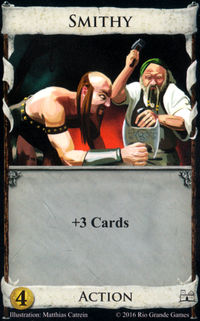
\includegraphics{dominion_smithy.jpg}
        
        The Smithy card when played allows the user
        to add three more cards to their hand from
        their pile. It costs four gold to purchase
        and takes one action to use. 
      \item \textbf{Handled in Code}

        Within the cardEffect function, if this
        card is activated, the code will
        call drawCard(currentPlayer, state)
        three times and then call
        discardCard(handPos, currentPlayer, state, 0)
        and return. 

        drawCard() will update information about the
        gamestate as well as the player information. 
        It will check if the current deck is empty,
        and if so it will shuffle the discard pile
        back into the deck. Then, it will draw a card 
        and add that card to the player's hand.

        discardCard() will first check whether to
        trash the card rather than discard the
        card. The only difference between trashing
        and discarding as a matter of game
        mechanics is that trashed cards are 
        discarded face up so that all other players
        can view what was discarded. discardCard()
        tracks which card to discard by referencing
        the index of the card in the player's hand, 
        which is a variable stored in the gameState
        of the game. The function will 
        appropriately update the number of cards in
        the player's hand and it will update the
        positions of the cards. 

    \end{itemize}

  \item Adventurer
    \begin{itemize}
      \item \textbf{Explanation}

        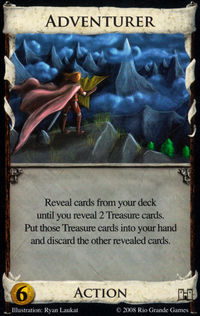
\includegraphics{dominion_adventurer.jpg}
        
        The adventurer card lets the player 
        reveal the top card of the the deck until
        two treasures are found. The two treasures
        are added to the player's hand and the
        other revealed cards are discarded. 
        
      \item \textbf{Handled in Code}
      
        If the adventurer card is played, then within
        the cardEffect function, the adventurer case
        is activated. First, the a while loop will
        check whether drawnTreasure is less than two,
        and drawnTreasure is an integer initialized to
        0. Then, it will shuffle the discard back into
        the deck if the deck is empty. Afterwards, it
        will call drawCard. It will check the last
        card drawn, which is a variable stored in
        the current state of the game. It will 
        increment drawnTreasure only if the drawn
        treasure is a copper, silver, or gold. If not, 
        then it will remove the top card in the player's 
        hand, which has the effect of discarding any non
        treasure card. 

    \end{itemize}

  \item Council Room
    \begin{itemize}
      \item \textbf{Explanation}

        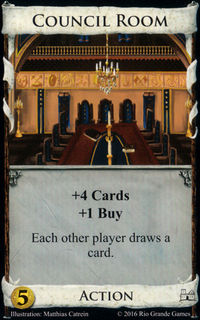
\includegraphics{dominion_councilroom.jpg}

        This card lets the player draw four cards and increments
        their buys by 1. It also draws one card each for every
        other player. It costs five gold to purchase. 

      \item \textbf{Handled in Code}
        
        The code first calls drawCard four times for the 
        currentPlayer. Then, it updates the numBuys variable
        stored in the gamestate. Then, it loops through the 
        number of players (each player is assigned an integer
        from 0 to n -1 where n is the number of players) and
        it calls drawCard
        for the ith player only if that player is not
        the currentPlayer. It will discard the current card
        and return.

    \end{itemize}

  \item Village
    \begin{itemize}
      \item \textbf{Explanation}

        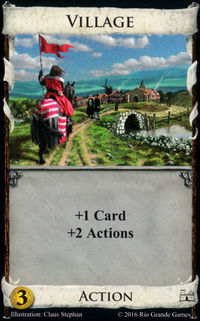
\includegraphics{dominion_village.jpg}

        This card will draw one card for the current player
        and increase the player's actions by two. Costs three
        gold to purchase. 

      \item \textbf{Handled in Code}

        The village case will call drawCard for the current 
        player, increment the numActions variable of the
        gameState object by two, and then discard itself. 
    \end{itemize}

  \item Great Hall
    \begin{itemize}
      \item \textbf{Explanation}

        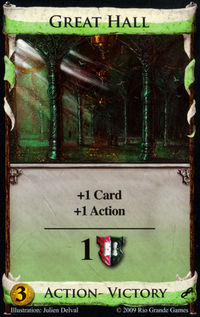
\includegraphics{dominion_greathall.jpg}

        This card will draw another card for the player, increase
        the number of actions they can play, and it will also
        increase the total victory points they have acrued thus
        far in the game.

      \item \textbf{Handled in Code}
      
        The code will call drawCard to add another card to the player's 
        hand, it will access the gameState object to increment the
        numActions variable, and it will then discard. The game handles
        the counting of victory points at the end where it will count
        this card in any player's hand towards the total. 
    \end{itemize}
\end{enumerate}
\end{document}
